\section{Mikrocontroller}
\label{ref_adc}
Til  styring af robotten har gruppen valgt at anvende et UCN board. Dette besidder 128 kb flash memory og 16 pins til in- og output. Fem af disse er analoge pins som fungere i et spændingsinterval mellem 2.3-3.6 V. 
\newline
Deruover har UCN boardet to UART pins (hardware serial ports). Disse har gruppen valgt at anvende under test af ADC\ref{ref_adc} for at verificere at ADC'en virker efter hensigten. 
Til mikrocontrolleren anvendes et motorshield hvilket muliggør anvendelsen af flere pins samt stying af de påmonteret DC motorer på Sparkfun's Magician Chassis.
\newline 
UCN boardet's mikroprocessor er en pic32mx250f128b som er en del af pic32 familien og har en maks clock frekvens på 50MHz. 
Strømmen tilføres mikrokontroller via et 7.2 V. ekstern batteri gennem et Power Jack som er monteret på UCN boardet's PCB(Printed circuit board). 

\begin{figure}[h!]
  \centering
  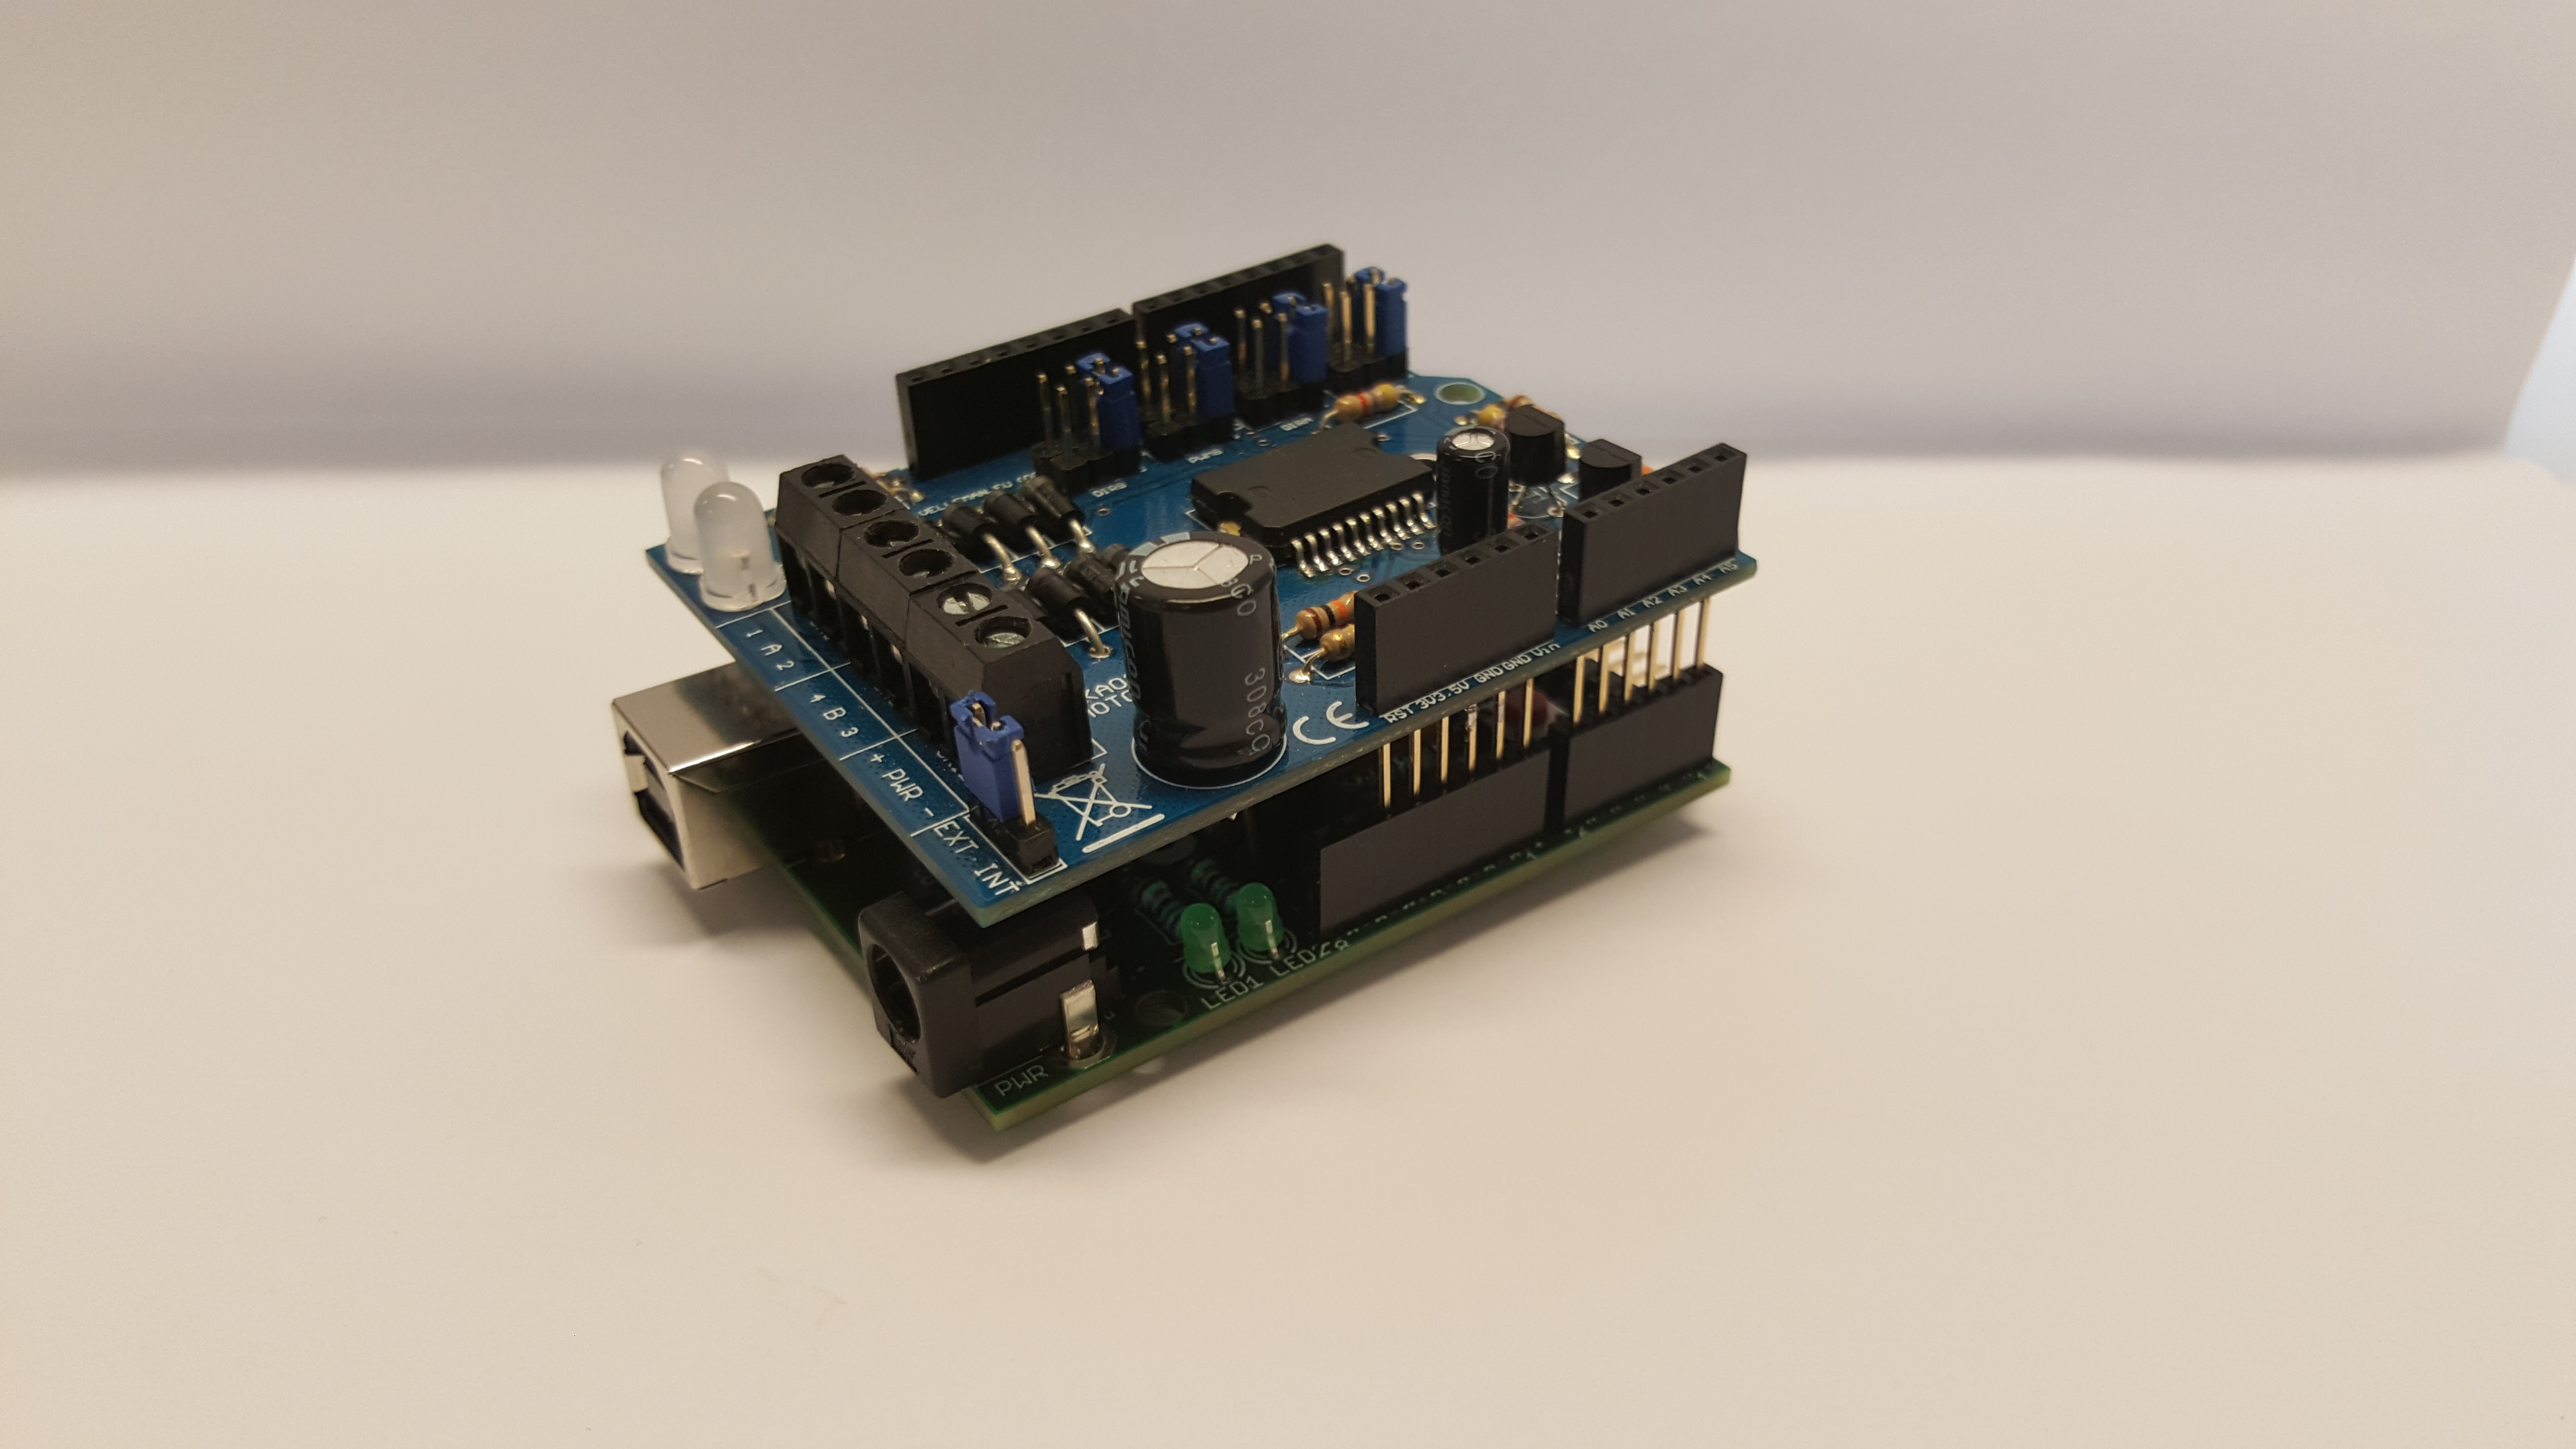
\includegraphics[width=0.6\textwidth]{figures/arduinoMshield.png}
  \caption{UCN board med påmonteret motorshield til styring af robotten.}
  \label{arduino&shield}
\end{figure}

\newpage
